% !TEX root = ../main.tex
\section{Figures and tables}
\label{sec:figures}

This section checks figures from the figures/ folder, subfigures, tables and multiple columns.

\Cref{fig:oscillator} is a PDF file in figures/, produced by the Python script next to it, figures/damped-oscillator.py.
If it appears, the graphics path works.
Its label should read Fig. in bold followed by a period.

\begin{figure}[H]
   \centering
   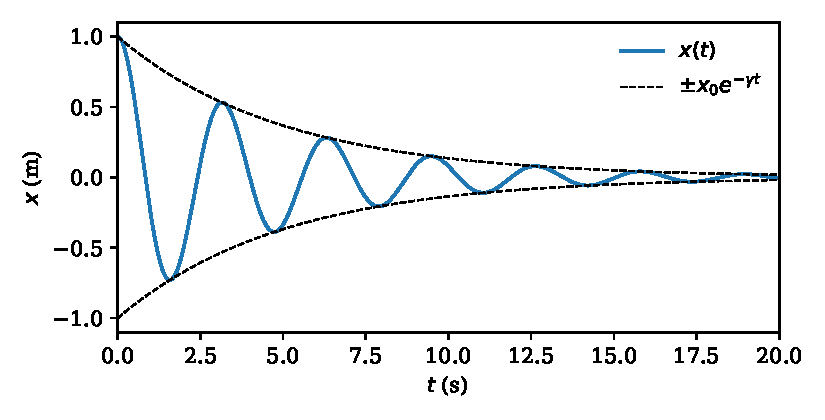
\includegraphics[width=0.75\linewidth]{damped-oscillator}
   \caption{Position of the damped oscillator, \cref{eq:solution}, with the parameters of \cref{tab:parameters}. The dashed lines are the envelope $\pm x_0 e^{-\gamma t}$.}
   \label{fig:oscillator}
\end{figure}

\Cref{fig:subfigures} has two subfigures that can be referenced separately, as \cref{fig:sub-a} and \cref{fig:sub-b}.
The images are placeholders that come with TeX Live.

\begin{figure}[htbp]
   \centering
   \begin{subfigure}{0.4\linewidth}
      \centering
      \includegraphics[width=\linewidth]{example-image-a}
      \caption{First subfigure.}
      \label{fig:sub-a}
   \end{subfigure}
   \hfill
   \begin{subfigure}{0.4\linewidth}
      \centering
      \includegraphics[width=\linewidth]{example-image-b}
      \caption{Second subfigure.}
      \label{fig:sub-b}
   \end{subfigure}
   \caption{Two subfigures in one figure.}
   \label{fig:subfigures}
\end{figure}

\Cref{tab:parameters} uses booktabs rules and siunitx columns, so the numbers are aligned on the decimal point.

\begin{table}[htbp]
   \centering
   \caption{Parameters used in \cref{fig:oscillator}.}
   \label{tab:parameters}
   \begin{tabular}{l c S[table-format=1.3] l}
      \toprule
      Quantity & Symbol & {Value} & Unit \\
      \midrule
      Mass & $m$ & 1.0 & \unit{kg} \\
      Spring constant & $k$ & 4.0 & \unit{N/m} \\
      Damping coefficient & $b$ & 0.4 & \unit{kg/s} \\
      Initial position & $x_0$ & 1.0 & \unit{m} \\
      Damped angular frequency & $\omega_d$ & 1.990 & \unit{rad/s} \\
      \bottomrule
   \end{tabular}
\end{table}

The last check is the multicol package.
The following paragraph should be split into two columns.

\begin{multicols}{2}
With $m = \qty{1.0}{kg}$, $k = \qty{4.0}{N/m}$ and $b = \qty{0.4}{kg/s}$, \cref{eq:definitions} gives $\omega_0 = \qty{2.0}{rad/s}$ and $\gamma = \qty{0.2}{s^{-1}}$.
Then \cref{eq:omega-d} gives $\omega_d = \sqrt{4.00 - 0.04}\,\unit{rad/s} = \sqrt{3.96}\,\unit{rad/s} \approx \qty{1.990}{rad/s}$.
The amplitude decays by a factor $e$ in a time $1/\gamma = \qty{5}{s}$, which is the scale visible in \cref{fig:oscillator}.
If this text is in two balanced columns, everything in the template works.
\end{multicols}
